\documentclass[twocolumn]{article}

\usepackage{geometry}
\geometry{textwidth = 18cm,textheight = 24cm}

\usepackage{cite}
\usepackage{caption}
\usepackage{graphicx}
\usepackage{amsmath}
\usepackage{amssymb}
\usepackage{textcomp}
\usepackage{lmodern}
\usepackage{authblk}
  
\title{Fluxonic processing of photonic synapse events}
\author[1]{Jeffrey M. Shainline}
%\author[2]{someone else}
\affil[1]{National Institute of Standards and Technology, Boulder, CO, 80305}
%\affil[2]{somewhere else}
\date{\today}
\setcounter{Maxaffil}{0}
\renewcommand\Affilfont{\itshape\small}

\begin{document}

\twocolumn[
  \begin{@twocolumnfalse}
    \maketitle
    \begin{abstract}
    Much of the information processing performed by a neuron occurs in the dentritic tree. For neural systems using light for communication, it is advantageous to convert to the electronic domain at synaptic terminals so dendritic computation can be performed with electrical circuits. Here we present circuits based on Josephson junctions and mutual inductors that act as dendrites processing signals from synapses receiving single-photon communication events with superconducting detectors. We show simulations of circuits performing basic logical operations such as AND and OR, which become coincidence detectors when time dependence is added. These two-input logical operations straightforwardly extend to multiple inputs, and such a dendrites perform intermediate thresholding between the synapses and the cell body. We further show how the signal from a single-photon synapse event can fan out locally in the electronic domain by roughly a factor of ten to enable the dendrites of the receiving neuron to process in multiple different ways. Such a technique makes efficient use of photons and energy while providing access to significantly more information regarding an afferent spike train.
    \vspace{3em}
    \end{abstract}
  \end{@twocolumnfalse}
]

%\tableofcontents

\section{\label{sec:introduction}Introduction}
A neuron is a complex information processing device, integrating signals from thousands of inputs and producing pulses when those signals reach threshold. These pulses, referred to as neuronal firing events, consume the most energy of any operation in the network. The neurons receiving the pulses must extract as much information as possible from each pulse. Neurons accomplish this through processing occurring in synapses and dendrites. Because neural information is based on temporal sequences of pulses, the relevant processing involves applying various temporal filters to extract relevant data. For example, synapses perform temporal filtering of pulse trains to identify rising edges (high pass) and to identify pulse trains exceeding some duration or number of pulses (low pass) \cite{}. Dendrites receive and further process synaptic signals. The operations performed by dendrites include leaky integration \cite{}, identification of coincidences \cite{} and sequences \cite{haah2015} between synapses from different neurons, and intermediate nonlinear thresholding transfer functions between groups of synapses and the cell body \cite{}. Inhibitory neurons in the network can temporarily suppress the activity of a dendrite to dynamically isolate information of interest, thereby adapting the structural network into myriad functional networks.

For hardware to be efficient for neural information processing, these synaptic and dendritic operations must be efficiently manifest in the constituent devices. We have argued elsewhere that light is promising for communication in neural systems, and that utilization of superconducting single-photon detectors enables communication at the lowest possible light levels \cite{shbu2017}. Subsequent work introduced circuits transducing single-photon communication events to the electronic domain for subsequent information processing \cite{sh2018,sh2018_full}. References \cite{sh2018} and \cite{sh2018_full} discussed basic synaptic functionality, plasticity, neuronal integration, thresholding, and the production of light during a neuronal firing event. Here we extend that work to consider additional synaptic and dendritic computational functions thought to be important for neural information processing. We discuss three elemental circuits that can be used as building blocks to perform many neural operations. These operations include leaky integration and temporal filtering of afferent pulse trains, detection of coincidences between activities of input neurons, inhibition, and long-term memory retention of synaptic activity.

\begin{figure} 
    \centering{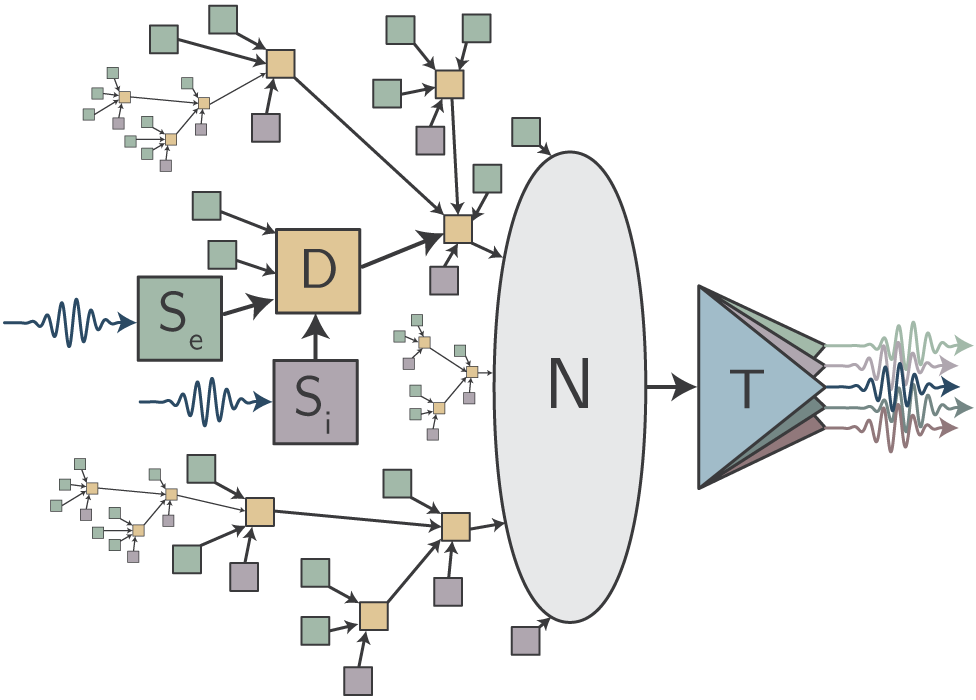
\includegraphics[width=8.6cm]{_01__schematic.png}}
	\captionof{figure}{\label{fig:schematic}Caption.}
\end{figure}
Reference \cite{sh2018} considered a simple model of neuronal operation wherein synapses directly connect to neurons, and each neuron performs leaky integration of the synaptic activities with a single decay time constant, $\tau$. Within that model, each neuron is capable of answering the question, ``Is the integral of activity across all synapses in the last $\tau$ seconds greater than threshold?'' If the answer is yes, the neuron produces a pulse. While such a model may be useful for certain neuromorphic computations, it assumes that each neuron ignores or is incapable of utilizing nearly all the information to which it has access. The purpose of this paper is to consider a more elaborate model for neural information processing in which the dentritic tree contains significantly more information about synaptic activities than a simple sliding sum. The model is illustrated schematically in Fig.\,\ref{fig:schematic}, which is intended to be an extension of a similar illustration used in Refs.\,\cite{sh2018} and \cite{sh2018_full}. We use the term, ``dentritic tree'' to refer to a neuron's input synapses and dendrites collectively, and Fig.\,\ref{fig:schematic} is intended to illustrate the potential complexity of the dentritic tree. In this work we develop circuits that will enable a neuron to answer subtle and varied questions, such as, ``How long has it been since neuron $i$ last produced a pulse?'' ``How many pulse trains have begun and then ceased on neuron $i$ in the last $\tau_i$ seconds?'' ``How many times have neurons $i$ and $j$ fired within $\tau_{ij}$ seconds of each other in the last $\tau_q$ seconds?''

\begin{figure} 
    \centering{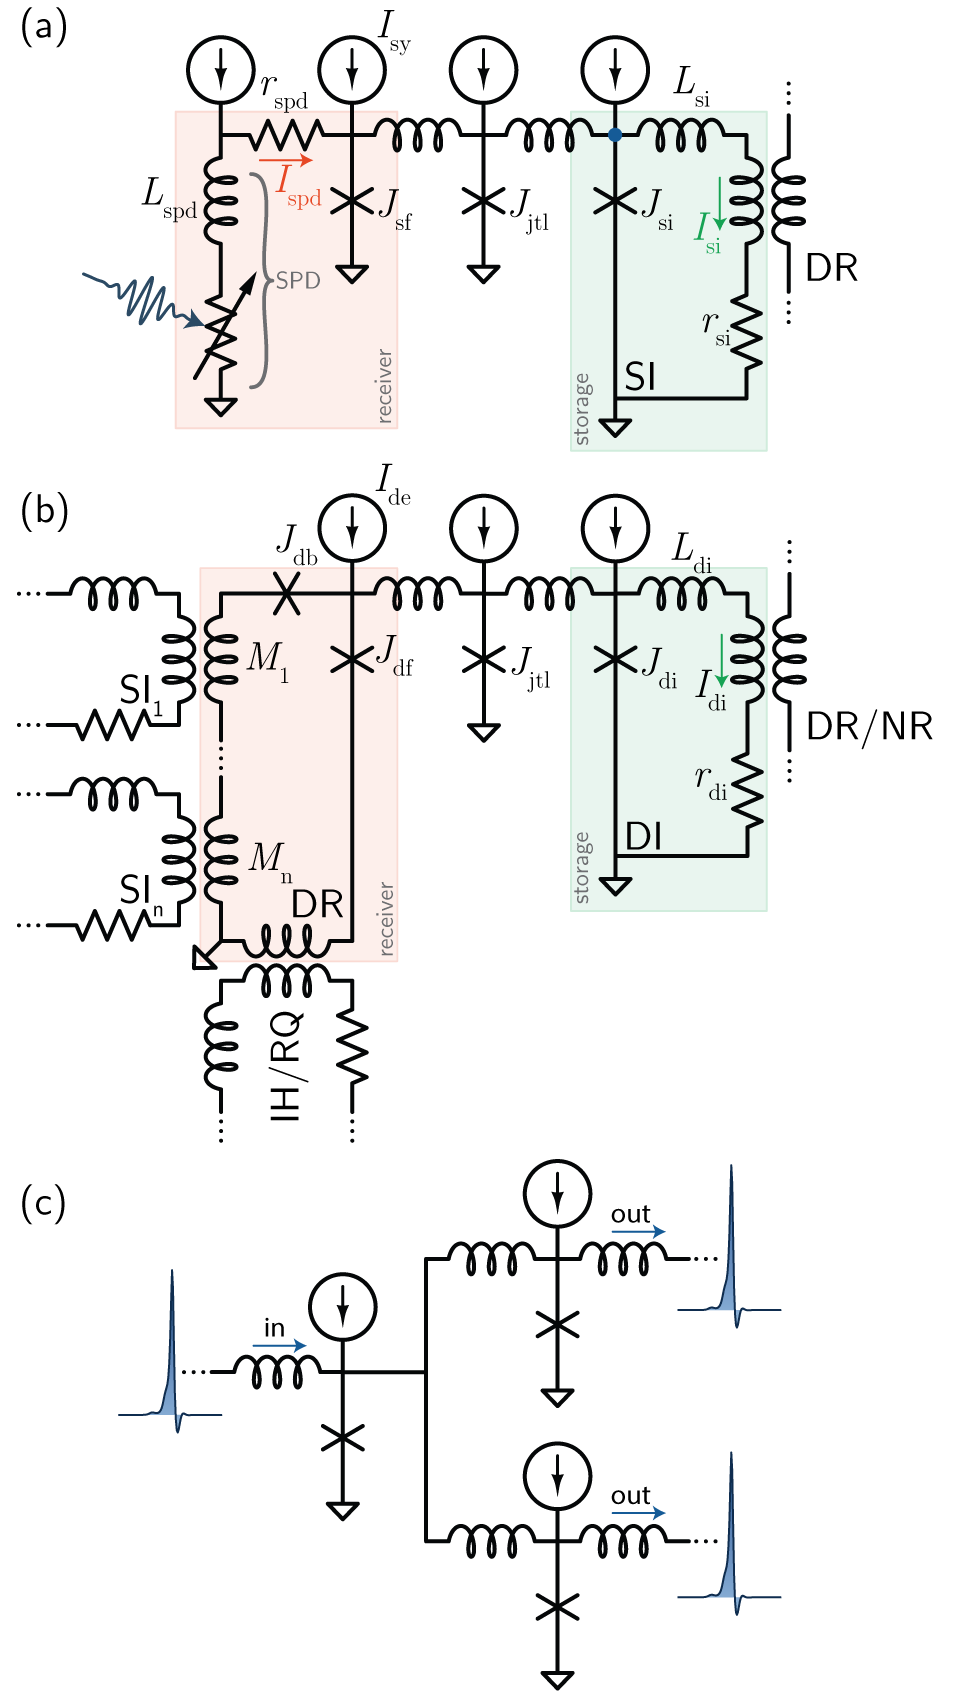
\includegraphics[width=8.6cm]{_02__circuits.png}}
	\captionof{figure}{\label{fig:circuits}Caption.}
\end{figure}
In this work, we introduce circuits based on mutual inductors and Josephson junctions capable of providing the answers to these questions. This work is entirely theoretical and is based on time-domain circuit simulations of the three elemental circuits shown in Fig.\,\ref{fig:circuits} when arranged in various configurations. In Sec.\,\ref{sec:synapse} we review the basic operations of a synapse that transduces a single-photon communication event to the superconducting electronic domain for information processing, and in Sec.\,\ref{sec:short_term} we consider operations performed on pulse trains at a single synapse, usually associated with short-term plasticity and synaptic computation \cite{abre2004}. In Sec.\,\ref{sec:correlations} we consider the detection of coincidences between two or more synapses, and we show how the same circuits can be used with broken temporal symmetry to identify sequences of activity. In order for these various pieces of information to be utilized only when relevant, inhibition can be used to silence specific dendrites at appropriate times. Alternatively, it is possible to instead set a dendrite to silence by default, and provide access to its contents only at appropriate times. To accomplish this, we introduce a new type of dendritic readout that we refer to as rapid query, and we posit the utility of a dedicated class of rapid query neurons that, upon firing, ask question of sets of dendrites and cause those dendrites to report the answers to those questions up the dendritic tree toward the neuron cell body. Inhibition and rapid query are discussed in Sec.\,\ref{sec:inhibition_and_rapid_query}. 

A central premise of the body of work represented by Refs.\,\cite{shbu2017,sh2018,sh2018_full,sh2018_ICRC} is that scalable neural systems will benefit from the fan-out and efficiency of few-photon communication. Yet when superconducting electronic circuits are employed for computation, these few-photon communication events dominate the energy budget. In Sec.\,\ref{sec:fluxonic_fanout} we discuss the use of superconducting splitters to make copies of photonic synapse events to that all of the questions discussed above can be answered by the dentritic tree through processing of the signal from a single photon. Thus, the proposed hardware aspires to achieve greater than one-to-one-thousand fan-out in the photonic domain from each neuron to its thousands of connections. Subsequently, at each neuronal terminal, the hardware aspires to achieve an additional factor of roughly one-to-ten fan-out in the electronic domain, providing each receiving neuron with the capability of analyzing much more information about the synaptic activity. All fan-in occurs in the electronic domain as the dentritic tree feeds its signals into the neuron cell body. Section \ref{sec:discussion} contains a discussion of the results.

\section{\label{sec:synapse}Photon-to-fluxon transduction at a synapse}
\begin{figure} 
    \centering{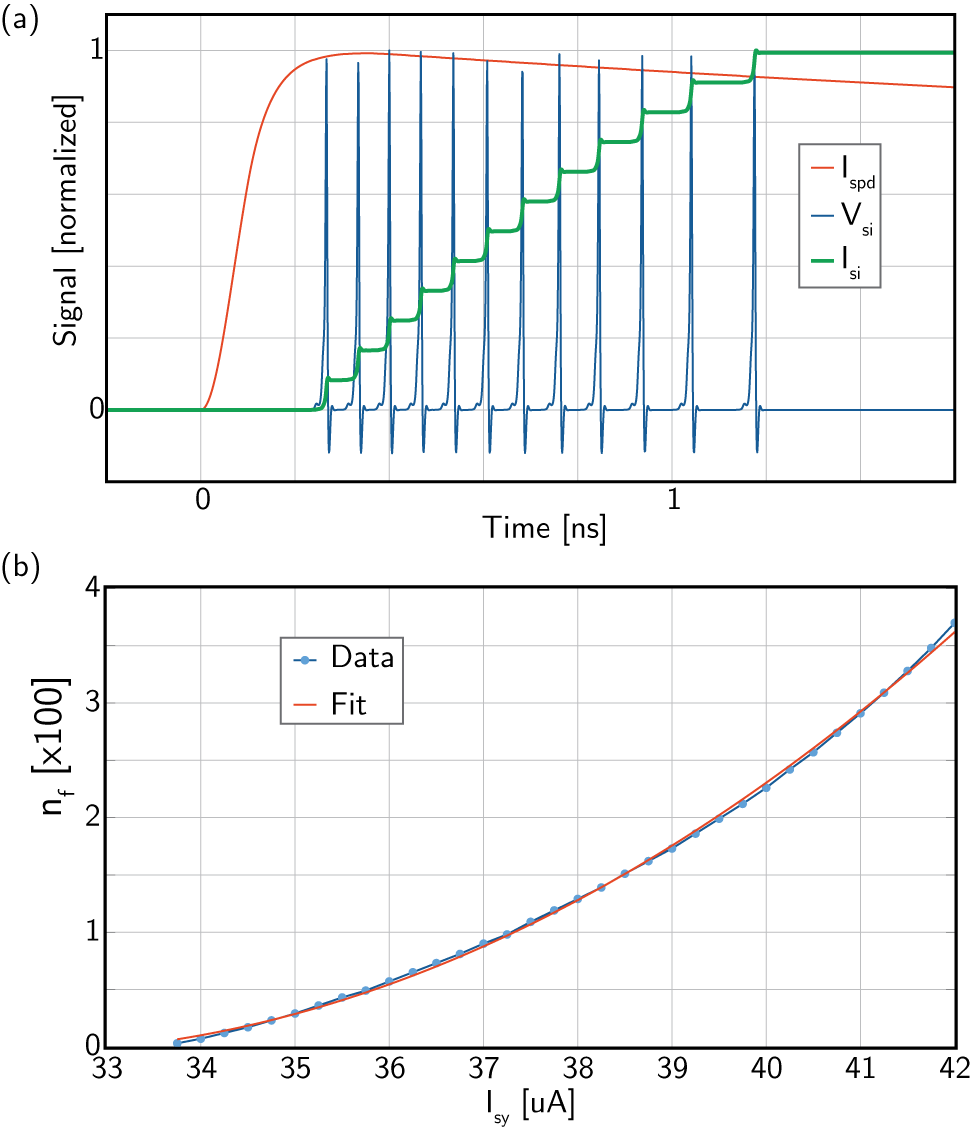
\includegraphics[width=8.6cm]{_03__sffg_basic.png}}
%        \setlength{\belowcaptionskip}{-20pt}
	\captionof{figure}{\label{fig:sffg_basic}Caption.}
\end{figure}
Analysis of fluxonic processing of photonic synapse events begins with consideration of the circuit that transduces a single-photon detection event to the superconducting electronic domain in the form of a series of fluxons. The circuit that accomplishes this is shown in Fig.\,\ref{fig:circuits}(a). This circuit was first introduced in Ref.\,\cite{sh2018} and described in more detail in Ref.\,\cite{sh2018_full}. The circuit comprises an initial receiver/transducer section, consisting of a superconducting-nanowire single-photon detector (SPD) \cite{gook2001,nata2012,liyo2013,mave2013} in parallel with a Josephson junction (JJ) \cite{ti1996,vatu1998,ka1999}. In the steady state, the SPD (drawn as a variable resistor in series with an inductor) has zero resistance, and thus its entire bias current flows directly through it to ground. The synaptic firing junction, $J_{\mathrm{sf}}$, is biased below its critical current ($I_{\mathrm{c}}$) by the synaptic bias current, $I_{\mathrm{sy}}$. Upon absorption of a photon, the variable resistor of the SPD switches temporarily to a high-resistance state ($\approx\,5$\,k$\Omega$) for a short duration ($\approx\,200$\,ps) \cite{yake2007}. The current through the SPD is diverted across a resistor ($I_{\mathrm{spd}}$ across $I_{\mathrm{spd}}$ in Fig.\,\ref{fig:circuits}(a)) and to $J_{\mathrm{sf}}$. At this point, the sum of the currents across $J_{\mathrm{sf}}$ exceeds $I_{\mathrm{c}}$, and the junction produces a series of fluxons \cite{ti1996,vatu1998,ka1999}. These fluxons propagate along the Josephson transmission line \cite{vatu1998,ka1999}, and are stored in the synaptic integration loop (SI). After the 200\,ps photon detection event, the bias current returns to the SPD with the time constant of $\tau_{\mathrm{spd}} = L_{\mathrm{spd}}/r_{\mathrm{spd}}$. This time constant has a minimum functional value determined by the electro-thermal properties of the nanowire \cite{yake2007}, and throughout this work we assume this time constant is fixed at $\tau_{\mathrm{si}} = 10$\,ns and the bias to the SPD is fixed at 10\,\textmu A. The number of fluxons created during a synaptic firing event depends on the net current across $J_{\mathrm{sf}}$ as well as the duration during which $J_{\mathrm{sf}}$ is biased above $I_{\mathrm{c}}$. With $\tau_{\mathrm{si}}$ and the bias to the SPD fixed, the number of fluxons, and thus the synaptic weight, are dynamically adaptable by changing the synaptic bias current, $I_{\mathrm{sy}}$. More details regarding $I_{\mathrm{sy}}$ and the associated plasticity mechanisms are given in Ref.\,\cite{sh2018_full}. 

The temporal activity of the circuit of Fig.\,\ref{fig:circuits}(a) during a synaptic firing event is shown in Fig.\,\ref{fig:sffg_basic}(a). Throughout this work, WRSpice \cite{wh1991} has been used to simulate all circuits, and all simulation parameters are given in the appendix. All JJs have $I_{\mathrm{c}} = 40$\,\textmu A and $\beta_{\mathrm{c}} = 0.95$. The red trace in Fig.\,\ref{fig:sffg_basic}(a) shows the current diverted from the SPD after a photon has been received. The blue trace shows the voltage pulses as the fluxons enter the SI loop. As each fluxon enters the loop, it introduces a discrete, fixed value of current given by $I_{\phi} = \Phi_0/L_{\mathrm{si}}$, where $\Phi_0 \approx 2\times10^{-15}$\,Wb is the magnetic flux quantum, and is $L_{\mathrm{si}}$ is the inductance of the synaptic integration loop. Throughout this work, we assume the value of $L_{\mathrm{si}}$ is chosen in design independently for each synapse and set in hardware at the time of fabrication. The green trace in Fig.\,\ref{fig:sffg_basic}(a) shows the increase in current as the fluxons enter the SI loop during a synaptic firing event. The discrete steps with each fluxon are evident, and the total amount of current added to the SI loop during a synaptic firing event depends on both the number of fluxons generated during the firing event (controlled dynamically by $I_{\mathrm{sy}}$) and the inductance of the SI loop (set in hardware as $L_{\mathrm{si}}$). 

The role of $I_{\mathrm{sy}}$ is to adapt the synaptic weight by changing the number of fluxons generated during a synaptic firing event. In Fig.\,\ref{fig:sffg_basic}(b) we show the number of fluxons generated during a synaptic firing event as a function of $I_{\mathrm{sy}}$. The fit shows close agreement with a second-order polynomial. This means of changing the synaptic weight has several important properties. First, it is slowly varying, so small changes in $I_{\mathrm{sy}}$ result in small changes in the synaptic efficacy. Second, the function is monotonic, so increases in $I_{\mathrm{sy}}$ always result in increased synaptic efficacy, while decreases in $I_{\mathrm{sy}}$ always result in decreases in synaptic efficacy. This is necessary to enable activity-based plasticity mechanisms \cite{somi2000,mage2012}, which have been explored in the context of these circuits in Ref.\,\ref{sh2018_full}. Third, the bias $I_{\mathrm{sy}}$ can be bounded so synaptic strength never exceeds a certain limit, and runaway activity is not possible. Finally, the integer number of fluxons generated can be made to cover a broad range so that analog synapses of relatively high bit depth can be achieved. Figure \ref{fig:sffg_basic}(b) shows that over eight bits (256 levels) can be utilized, and throughout this work we find the range of eight to 10 bits to be a comfortable working range for the circuits under consideration. This is, or course, much lower than the 64-bit processors used for high-arithmetic-depth numerical calculations. Yet neural computation benefits from performing lower-resolution operations with high efficiency with accuracy gained through redundancy and parallelism. 

\begin{figure} 
    \centering{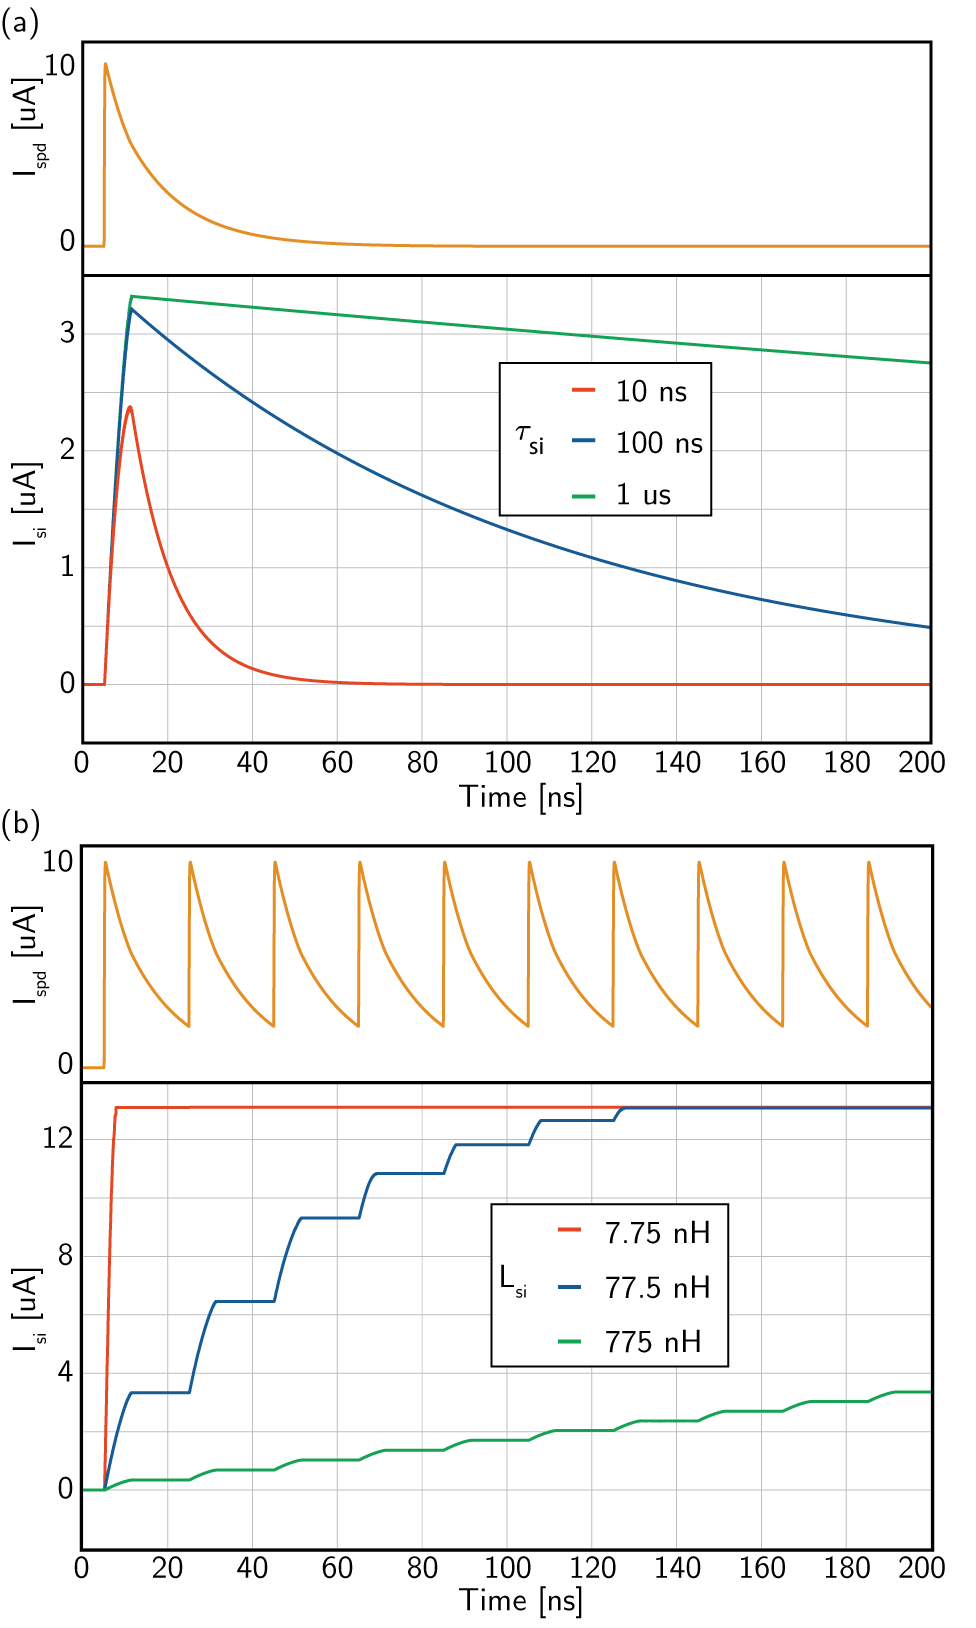
\includegraphics[width=8.6cm]{_04__sffg_betaL_tauSi.png}}
	\captionof{figure}{\label{fig:sffg_betaL_tauSi}Caption.}
\end{figure}
After a photonic communication event has been detected, the synaptic weight has been set as the number of fluxons created, and current has been added to the SI loop, further processing ensues. To start, the electrical current generated by the syanpse event can be stored for a chosen amount of time. This is determined by the leak rate of the SI loop, chosen in design and set in hardware by the time constant $\tau_{\mathrm{si}} = L_{\mathrm{si}}/r_{\mathrm{si}}$. Note that $\tau_{\mathrm{si}}$ is entirely independent of $\tau_{\mathrm{spd}}$, and because we consider superconducting circuits a memory of a synaptic event can persist indefinitely. Also note that while  the amount of current added to the SI loop during a synaptic firing event depends on $L_{\mathrm{si}}$, $r_{\mathrm{si}}$ can be chosen independently from $L_{\mathrm{si}}$, thereby enabling the amount of current and its storage time to separately selected. In Fig.\,\ref{fig:sffg_betaL_tauSi}(a) we show the temporal decay of current in the SI loop following a single synaptic firing event. The current can be released quickly, on the order of the SPD reset time of 10\,ns, or it can be stored 10 or 100 times longer to retain a memory of the event for as long as required. Here we show decay times spanning two orders of magnitude\textemdash from 10\,ns to 1\,\textmu s\textemdash, and it is likely that synaptic event retention times longer than this will not be necessary, as longer-term information storage is accomplished by modifying the plastic synaptic weight. 

%move this paragraph above previous paragraph
In biological neural systems, processing among local clusters of neurons occurs primarily through fast activity in the range of gamma frequencies (30\,Hz - 80\,Hz \cite{budr2004,bu2006}). This frequency range emerges because it reaches the upper limit of speed for the excitatory pyramidal neurons participating in the activity. In the superconducting optoelectronic hardware under consideration, this upper speed limit is near 100\,MHz, limited by the 10\,ns reset time of the SPDs in the synapses and of the transmitter circuits that generate neuronal firing events \cite{sh2018_full}. Therefore, we expect the neurons under consideration to demonstrate behavior similar to gamma oscillations, bursting with inter-spike intervals on the order of 10\,ns. Similarly, biological neural systems process information across the network as a whole through slower activity at theta frequencies of 4\,Hz - 8\,Hz \cite{budr2004,bu2006}. Naively mapping this scaling onto the system under consideration, we pay particular attention to gamma oscillations occurring at 100\,MHz as well as theta oscillations occurring at 10\,MHz. It is for this reason that we have considered the values of $\tau_{\mathrm{si}}$ in Fig.\,\ref{fig:sffg_betaL_tauSi}(a), and based on these consideration we must also consider the behavior of a synapse in response to a spike train corresponding to spike trains at gamma frequencies. 

We next consider the saturation of a synaptic integration loop, as shown in Fig.\,\ref{fig:sffg_betaL_tauSi}(b). As stated above, the current associated with a fluxon being generated in a loop of inductance $L$ is $I_{\phi} = \Phi_0/L$. This current circulates in the opposing direction of the applied bias to the JJ. The number of fluxons that can enter the loop before the cumulative opposing bias equals $I_{\mathrm{c}}$ is given by $I_{\mathrm{c}}/I_{\phi} = L I_{\mathrm{c}}/\Phi_0 = \beta_{\mathrm{L}}/2 \pi$, where $\beta_{\mathrm{L}}$ is a common parameter quantifying the flux storage capacity of a superconducting loop, and thus $\beta_{\mathrm{L}}/2\pi$ quantifies the number of fluxons that each add a $2\pi$ phase shift to the JJ. $\beta_{\mathrm{L}}/2\pi$ gives an estimate for how many fluxons a given SI loop will be able to store before saturation, and the exact number depends on the bias to $J_{\mathrm{si}}$ as well as the inductance to the left of $J_{\mathrm{si}}$ in Fig.\,\ref{fig:circuits}(a), which determines the added bias to $J_{\mathrm{si}}$ each time a fluxon is incident upon the junction due to a synaptic firing event. 

In Fig.\,\ref{fig:sffg_betaL_tauSi}(b) we show the integrated current in an SI loop as a function of time in response to a periodic train of pulses with 10\,ns inter-spike interval. Here we fix $\tau_{\mathrm{si}} = \infty$ and vary the inductance of the loop, $L_{\mathrm{si}}$, which changes the amount of current added to the loop with each fluxon and therefore each synaptic firing event. In these simulations, the value of $I_{\mathrm{sy}}$ was fixed at 38\,\textmu A, so 129 flux quanta are generated during the synaptic firing event. With a small value of $L_{\mathrm{si}}$, the quantity $\beta_{\mathrm{L}}/2\pi = L_{\mathrm{si}} I_{\mathrm{c}}/\Phi_0 =  150$, and the loop saturates after a single synaptic firing event. With an intermediate value of $L_{\mathrm{si}} = 77.5$\,nH, $\beta_{\mathrm{L}}/2\pi = 1.5\time 10^3$, and seven synaptic firing events fill the loop. With a large value of $L_{\mathrm{si}} = 775$\,nH, $\beta_{\mathrm{L}}/2\pi = 1.5\times 10^{4}$, and the loop can hold the activity from nearly 100 synaptic firing events with this value of $I_{\mathrm{sy}}$. Figure \ref{fig:sffg_betaL_tauSi}(b) shows the control one has in design over the capacity of the SI loop. The loop can operate as a binary device switching from a low to high state with each synapse event, or it can act as an analog device capable of representing many synapse events with distinct values of current. This saturation is a simple form of nonlinearity present in the synapse. The two parts of Fig.\,\ref{fig:sffg_betaL_tauSi} illustrate the two basic degrees of freedom of the SI loop: the signal storage time and storage capacity. We now proceed to explore the use of such synapses to extract information from pulse trains.

\section{\label{sec:short_term}Operations on pulse trains at a single synapse}
\begin{figure} 
    \centering{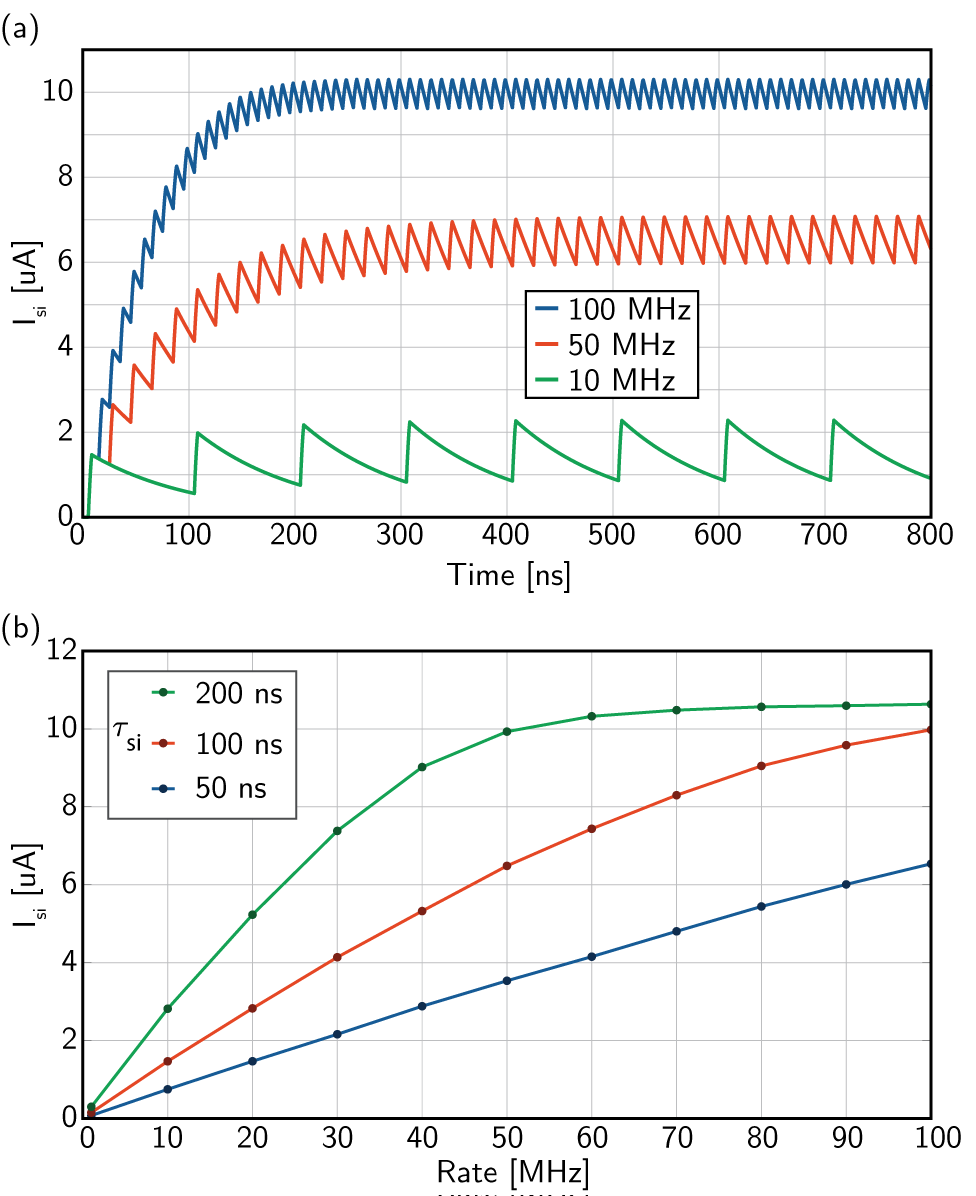
\includegraphics[width=8.6cm]{_05__sffg_rate_conversion.png}}
	\captionof{figure}{\label{fig:sffg_rate_conversion}Need description of averaging procedure (see pg 65 in green)}
\end{figure}
As an example of one form of processing that can be performed using the synaptic circuit of Fig.\,\ref{fig:circuits}(a), Fig.\,\ref{fig:sffg_rate_conversion} considers the operation of rate-to-current conversion. The first term of the Volterra expansion of a spike train corresponds to the time-averaged spike rate \cite{geki2002}, so a neuron must be able to decode this information. This can be accomplished with the synaptic transducer of Fig.\,\ref{fig:circuits}(a) when the SI loop is given a leak rate, as discussed in the context of Fig.\,\ref{fig:sffg_betaL_tauSi}(a). The circuit behaves as a standard leaky integrator, so the current in the SI loop obeys
\begin{equation}
\label{eq:leaky_integrator}
\frac{dI_{\mathrm{si}}}{dt} = \alpha-\frac{I_{\mathrm{si}}}{\tau_{\mathrm{si}}},
\end{equation}
where $\alpha = n_{\mathrm{f}} \Phi_0 R/L_{\mathrm{si}}$ with $n_{\mathrm{f}}$ the number of fluxons produced in each synaptic firing event and $R$ the rate of afferent synaptic activity. Equation \ref{eq:leaky_integrator} has the steady-state solution $I_{\mathrm{si}} = \alpha \tau_{\mathrm{si}}$, indicating that the current in the loop is proportional to the rate of input spikes. In Fig.\,\ref{fig:sffg_rate_conversion}(a) we show temporal traces of the current $I_{\mathrm{si}}$ in the presence of afferent activity at various rates for a loop with $\tau_{\mathrm{si}} = $100\,ns and $L_{\mathrm{si}} = $77.5\,nH. The value of $I_{\mathrm{si}}$ reaches a steady-state value when averaged over a time longer than the period of incoming pulses. The linear rate-to-current conversion holds as long as the integration time of the loop is short enough to avoid saturation, that is, $\alpha \tau_{\mathrm{si}} < I_{\mathrm{si}}^{\mathrm{sat}}$. In Fig.\,\ref{fig:sffg_rate_conversion}(b) we show the time-averaged current, $\bar{I_{\mathrm{si}}}$, as a function of the synaptic firing rate for three values of $\tau_{\mathrm{si}}$. With the value $\tau_{\mathrm{si}} = $50\,ns, the response is linear across the entire range of gamma and theta frequencies, while with the $\tau_{\mathrm{si}} = $200\,ns the loop reaches saturation, and higher input frequencies do not code unique information. If linear operation is desired, one must choose the time constant of the loop to be commensurate with the frequencies to be detected, or if nonlinear saturation is desired, longer integration times can be utilized. If increased dynamic range is advantageous, one can utilize the splitter of Fig.\,\ref{fig:circuits}(c) to activate multiple SI loops with different time constants from the same photonic synapse, as described in Sec.\,\ref{sec:fluxonic_fanout}.

The synaptic transducer and SI loop of Fig.\,\ref{fig:circuits}(a) on its own can achieve straightforward rate-to-current conversion to make use of rate-coded neuronal information. Yet when $I_{\mathrm{si}}$ is coupled to the circuit of Fig.\,\ref{fig:circuits}(b) through a mutual inductor, significantly more functionality can be achieved. Let us first describe the basic operation of the circuit, which we refer to as a dendritic processing circuit or dendrite. The dendritic processing circuit of Fig.\,\ref{fig:circuits}(b) is similar to the synaptic transducer circuit of Fig.\,\ref{fig:circuits}(a). Unlike the synapse, which receives photonic input, the dendrite receives input as flux coupled through mutual inductors. In the steady state, all junctions are biased below $I_{\mathrm{c}}$. Afferent input to the dendritic receiving (DR) loop from one or more SI loops increases the bias to the dendritic firing junction ($J_{\mathrm{df}}$) and decreases the bias to the dendritic buffer junction ($J_{\mathrm{db}}$). When the net bias to $J_{\mathrm{df}}$ exceeds $I_{\mathrm{c}}$, one or more fluxons will be produced, they will traverse the JTL, and they will add flux to the dendritic integration (DI) loop, just as in the case of the synapse. 

The main computational attributes of the dendrite come from the biasing conditions and interplay between $J_{\mathrm{df}}$ and $J_{\mathrm{db}}$. If the biases are established such that when $J_{\mathrm{df}}$ produces a fluxon, the current added to $J_{\mathrm{db}}$ is insufficient to switch $J_{\mathrm{db}}$ until the added biases from the SI loop(s) decay, the device acts like a DC-to-SFQ converter (DCSFQ) \cite{vatu1998,ka1999}. $J_{\mathrm{df}}$ will produce exactly one fluxon, and the DR loop will then be inactivated until the counter bias across $J_{\mathrm{db}}$ due to the SI loop(s) decays, at which point $J_{\mathrm{db}}$ will produce a fluxon counter the one produced by $J_{\mathrm{df}}$, and the loop will be reset. In this configuration, the dendritic receiver has a binary character. If the net input exceeds threshold, it produces a fluxon, and it cannot produce another until the net bias drops below a reset value.

In the other mode of operation, the dendrite can produce a continuous stream of fluxons, much like the synaptic transducer. To achieve this operation, $J_{\mathrm{db}}$ is biased closer to $I_{\mathrm{c}}$ so that a fluxon generated by $J_{\mathrm{df}}$ is sufficient to switch $J_{\mathrm{db}}$. Thus, each time $J_{\mathrm{df}}$ produces a fluxon, it is rapidly canceled by $J_{\mathrm{db}}$, and the DR loop retains no net flux. $J_{\mathrm{df}}$ will continue to produce fluxons as long as it is held above $I_{\mathrm{c}}$, and in the presence of synaptic activation (current in one or more SI loops), a stream of fluxons will be generated by $J_{\mathrm{df}}$ and stored in the DI loop. Because this stream may contain any number of fluxons, we consider this the analog mode of operation.

Whether operating in binary or analog modes, the effect of the dendrite is to perform a nonlinear thresholding function on its inputs, and provide the output signal to the DI loop in the form of supercurrent. Just as in the SI loop, the DI loop can be configured to saturate rapidly (small $\beta_{\mathrm{L}}$) or store the signal from many threshold events (large $\beta_{\mathrm{L}}$), and the loop can be configured with a decay time constant ($\tau_{\mathrm{di}} = L_{\mathrm{di}} / r_{\mathrm{di}}$) spanning a broad range from time scales shorter than a gamma interspike interval to as long as superconductivity can be maintained. With these basic operating principles in mind, we proceed to elucidate the possibilities of dendritic processing with this circuit through examples.

We begin to explore the functions enabled by the dendritic processing circuit of Fig.\,\ref{fig:circuits}(b) by considering operations usually associated with synaptic computation \cite{abre2004}, namely short-term-facilitating and short-term-depressing plasticity. Some synapses are observed to provide no response or very weak response to the first pulse of a train, with the efficacy of the synapse increasing as the pulse train proceeds. This behavior is referred to as short-term facilitating plasticity, and it may be due to dynamics within the synapse itself or to the conductance properties of a dendrite or series of dendritic compartments. Here we simulate analogous behavior with a single synaptic transducer (Fig.\,\ref{fig:circuits}(a)) coupled to a single dendritic processing circuit (Fig.\,\ref{fig:circuits}(b)). To achieve this operation, we design an SI loop that can store the signals from multiple synaptic firing events without saturating, and we bias $J_{\mathrm{df}}$ so that the additional current induced by the first few synaptic firing events does not push the junction over $I_{\mathrm{c}}$, but after multiple synaptic firing events, $I_{\mathrm{c}}$ is exceeded and flux is added to the DI loop. We design the dendrite in analog mode for this behavior.

Circuit simulations of short-term-facilitating plasticity are shown in Fig.\,\ref{fig:si_di_facilitating}. Figure \ref{fig:si_di_facilitating}(a) shows the afferent pulse train. The first pulse occurs at 5\,ns, and the interspike interval is 20\,ns. Figures \ref{fig:si_di_facilitating}(b) and (c) show the accumulated current in the DI loop as a function of time. In all cases, at least three synaptic firing events are required before the bias across $J_{\mathrm{df}}$ exceeds $I_{\mathrm{c}}$ and current is added to the DI loop. In Fig.\,\ref{fig:si_di_facilitating}(b) the effect of the synaptic bias current, $I_{\mathrm{sy}}$ is shown. The primary effect of the dynamically reconfigurable bias current is to shift the curve left or right. With a stronger synaptic weight, more current will be added to the SI loop with each synaptic firing event, and therefore more current will be induced the the mutual inductor into the DR loop. Thus, fewer synaptic firing events are required to reach the dendritic threshold. In this example, $I_{\mathrm{sy}}$ can shift the threshold from eight to three synaptic firing events. In Fig.\,\ref{fig:si_di_facilitating}(c), the synaptic bias current is fixed at 38\,\textmu A, while the dendritic bias current, $I_{\mathrm{de}}$, is varied. Change in $I_{\mathrm{de}}$ has less of an effect on the number of pulses required to reach threshold, but it significantly affects the number of fluxons generated by $J_{\mathrm{df}}$ each time a synaptic firing event occurs, which is related to the slope of the traces in Fig.\,\ref{fig:si_di_facilitating}(c). The effect of the dendritic bias current, $I_{\mathrm{de}}$, is therefore analogous to the effect of the synaptic bias current, $I_{\mathrm{sy}}$. We therefore anticipate that $I_{\mathrm{de}}$ will provide a dynamically reconfigurable circuit parameter that can be used to establish a ``dendritic weight'' and can be used for long-term plasticity and learning. 
\begin{figure} 
    \centering{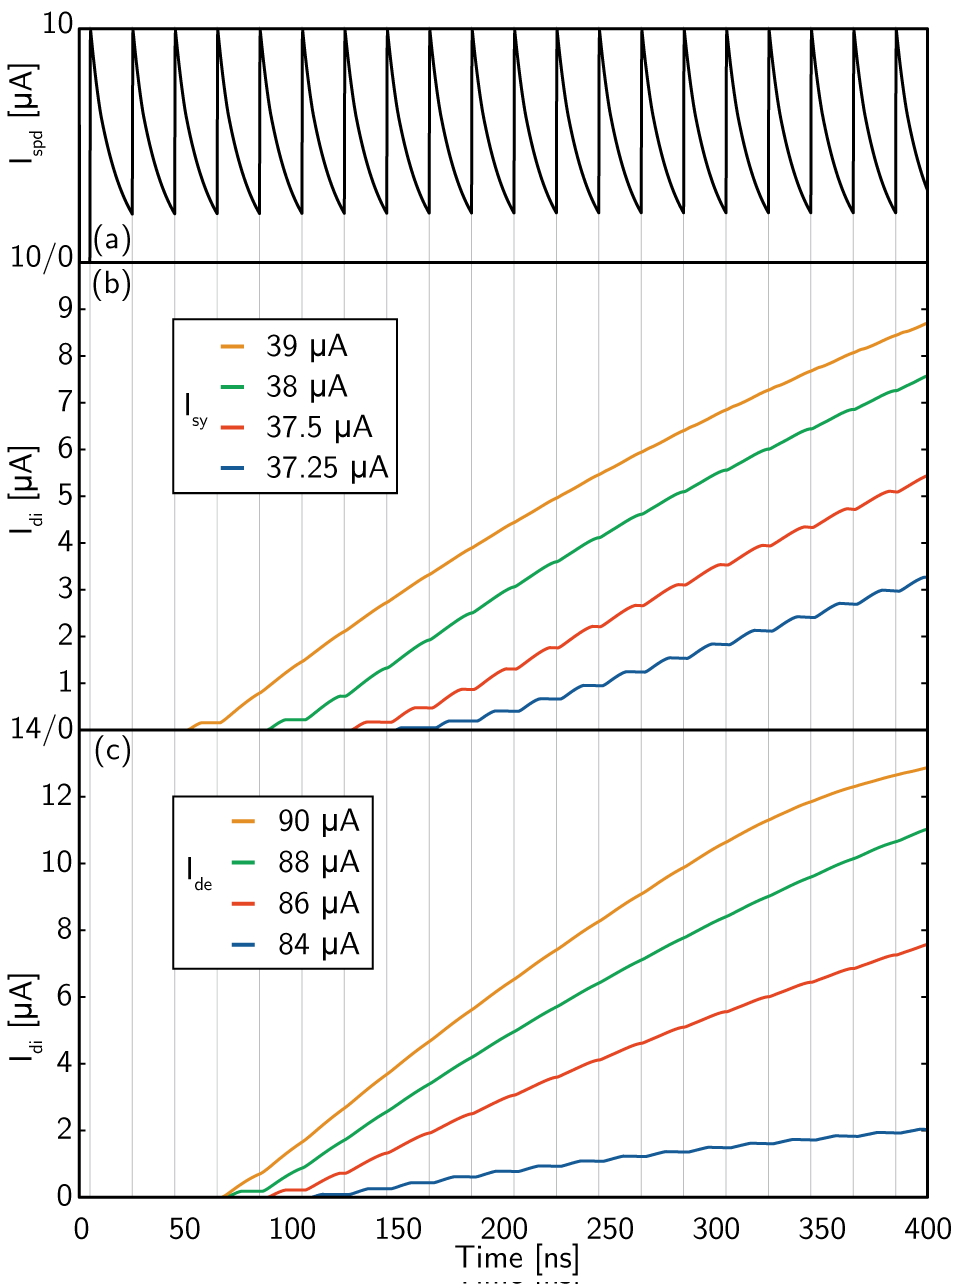
\includegraphics[width=8.6cm]{_06__si_di_facilitating.png}}
	\captionof{figure}{\label{fig:si_di_facilitating}Caption.}
\end{figure}

\begin{figure} 
    \centering{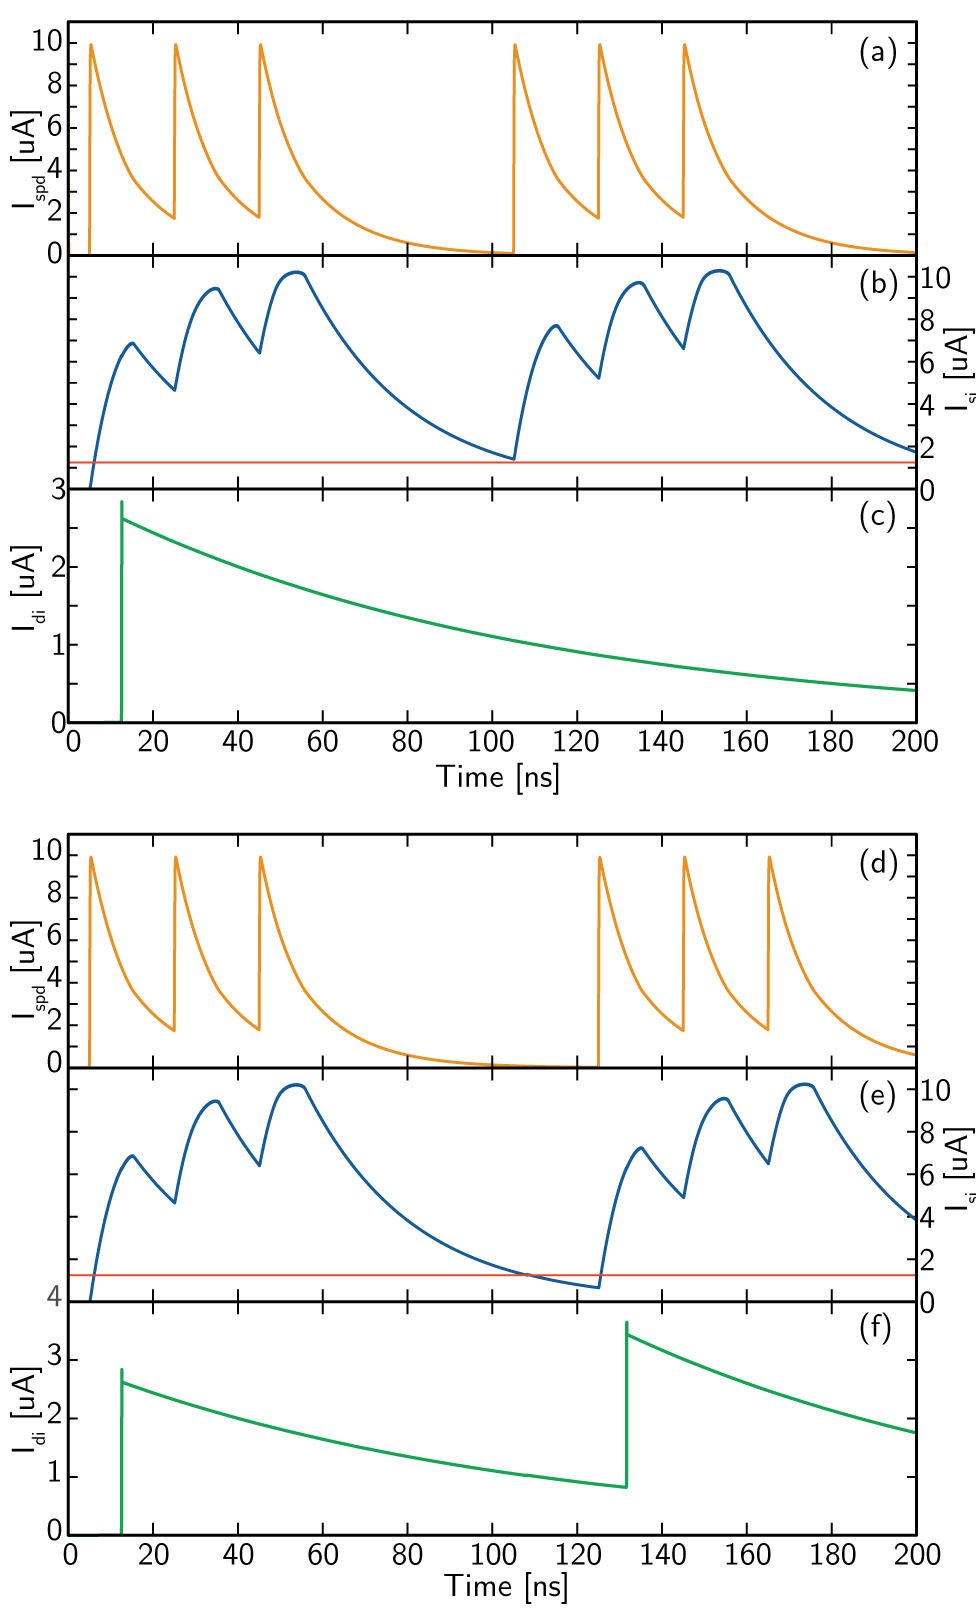
\includegraphics[width=8.6cm]{_07__si_dcsfq_depressing.png}}
	\captionof{figure}{\label{fig:si_dcsfq_depressing}Caption.}
\end{figure}
While facilitating behavior effectively strengthens a synapse as a pulse train proceeds, short-term-depressing plasticity gives the opposite behavior. In an extreme form, this mechanism can convey only the onset of a pulse train, while blocking subsequent spikes. To demonstrate this behavior, we consider the dendritic processing circuit in binary mode. Circuit simulations are shown in Fig.\,\ref{fig:si_dcsfq_depressing}. Consider first the upper panel, Fig.\,\ref{fig:si_dcsfq_depressing}(a-c). The current pulses from the SPD due to the afferent spike train are shown in Fig.\,\ref{fig:si_dcsfq_depressing}(a), and the resulting current in the SI loop is shown in Fig.\,\ref{fig:si_dcsfq_depressing}(b). The activity consists of two groups of three closely spaced spikes. The current in the DI loop is shown in Fig.\,\ref{fig:si_dcsfq_depressing}(c), and it is observed that a single pulse enters the DI loop at the onset of the first spike in the train. In Fig.\,\ref{fig:si_dcsfq_depressing}(b), we have marked with a red line the value of $I_{\mathrm{si}}$ below which reset occurs in the DR loop. We see that the first spike of the second group of three occurs just before $I_{\mathrm{si}}$ drops below the reset value. The second group of pulses is not identified as a new spike train, and so $I_{\mathrm{di}}$ continues decaying with $\tau_{\mathrm{di}}$ with no additional signal from the dendrite. By contrast, in the lower panel (Fig.\,\ref{fig:si_dcsfq_depressing}(d-f)), the onset of the second group of pulses occurs 20\,ns later that in the upper panel, giving the current in the SI loop time to decay below the reset value. In this case, when the second group of pulses begins, it is identified as a new train, and additional signal is added to the DI loop, again in the form of a single fluxon. The reset delay can be set in hardware across a broad range of values through $\tau_{\mathrm{si}}$ and can be adjusted over a smaller range dynamically through $I_{\mathrm{de}}$. Note that the dendritic receiving loop does not have any resistance of its own, so the current decay time constants in that loop are entirely determined by the SI loops. Also note that while we refer to this operation of the dendritic processing circuit as binary, the DI loop may be independently configured to store anywhere form one to many fluxons, providing the circuit as a whole with an analog representation of the number of afferent pulse trains occurring within a time period set by $\tau_{\mathrm{di}}$.

To summarize the operations we have investigated so far, the synaptic firing circuit on its own can accomplish rate-to-current conversion, reporting a temporal average of recent activity. By coupling the synaptic firing circuit to a dendritic processing circuit, we can construct a dendrite that generates signal only when a pulse train persists for a certain duration, reporting a low-pass-filtered spike train. We can use the same circuits with slightly different biasing configuration to construct a dendrite that generates signal only when a pulse train begins after a certain period of rest, reporting a high-pass-filtered spike train. All of these operations correspond to temporal filters performed on spike trains occurring at a single synapse. Yet an important function of dendritic processing is to identify correlations between the activities of multiple neurons. We now consider this task.

\section{\label{sec:correlations}Detecting correlations between neurons}
\begin{figure} 
    \centering{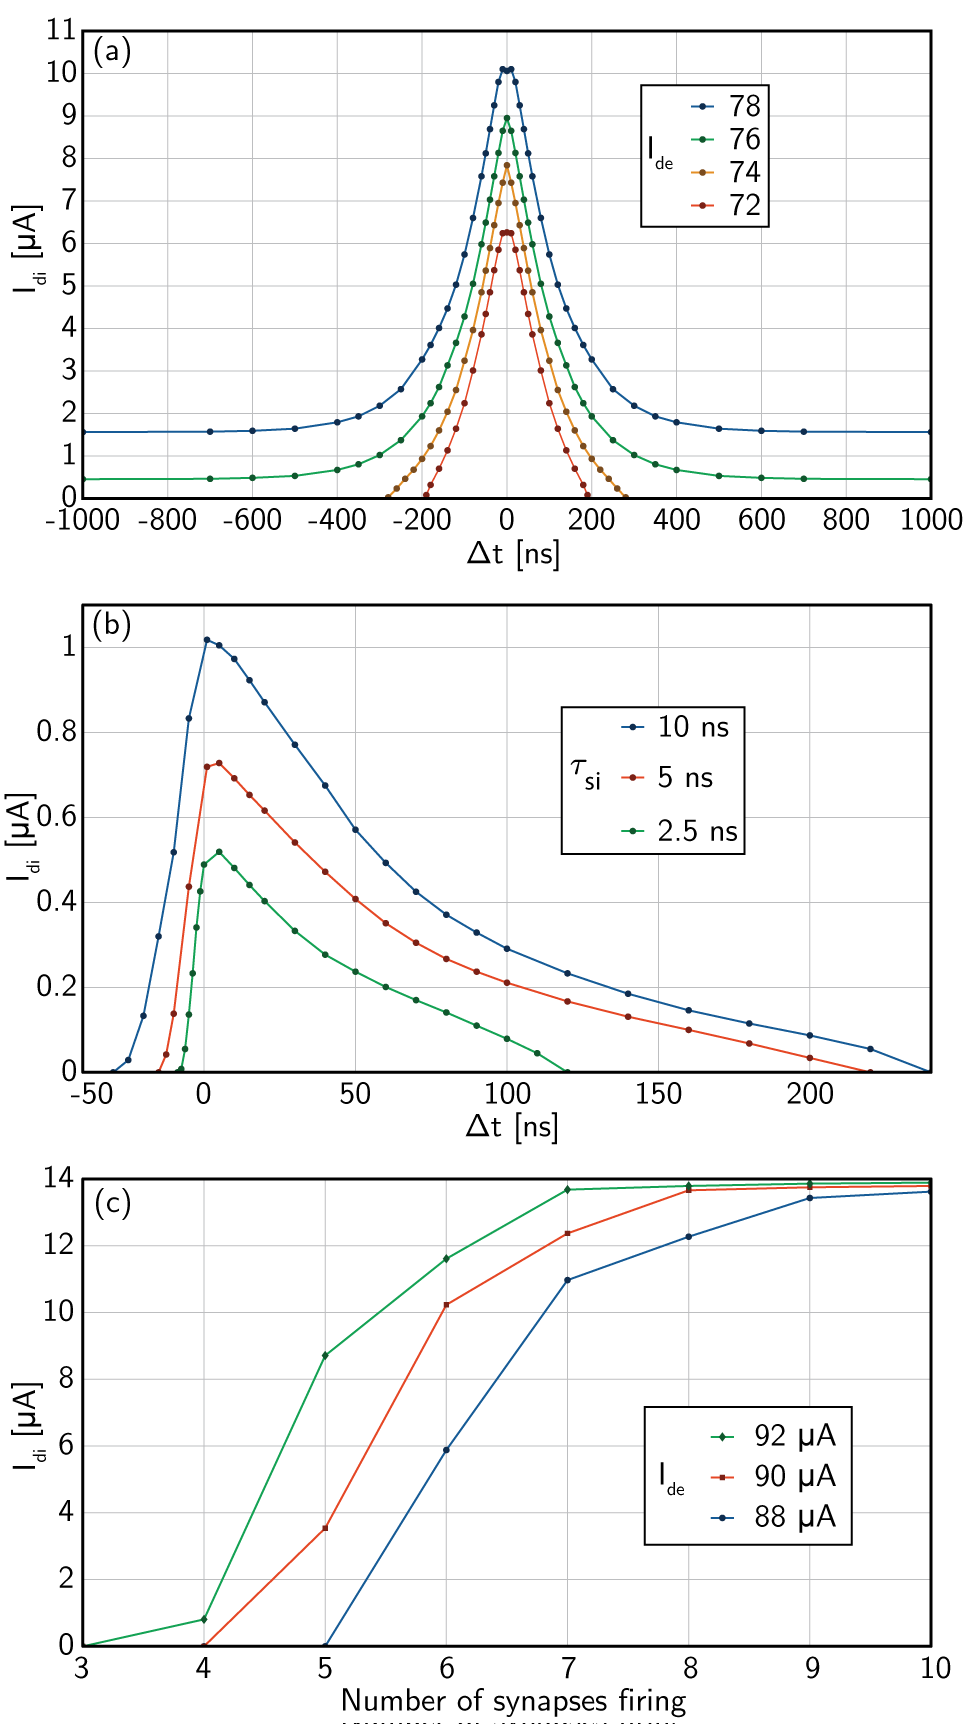
\includegraphics[width=8.6cm]{_08__poly_si_di.png}}
	\captionof{figure}{\label{fig:poly_si}Caption.}
\end{figure}
The second term in a Volterra expansion of the activities of two neurons corresponds to coincidences between the two neurons. We can use the same dendritic processing circuit of Fig.\,\ref{fig:poly_si} to detect coincidences, provided two SI loops are coupled to the DR loop through mutual inductors. In the simplest case, we wish to know whether two synapses have fired within a certain time period. This can be achieved by giving both SI loops the same value of $\tau_{\mathrm{si}}$. The response of such a circuit is shown in Fig.\,\ref{fig:poly_si}(a), where the current induced in the DI loop is shown as a function of the time delay between the two synaptic firing events for several values of $I_{\mathrm{de}}$ with $\tau_{\mathrm{si}} =$100\,ns. For the two lower values of $I_{\mathrm{de}}$, the circuit can be thought of as an AND gate with an analog extension to the time domain: if synapse $i$ AND synapse $j$ fire within a time period set by $\tau_{\mathrm{si}}$, a signal dependent on the time difference is added to the DI loop. For larger values of $I_{\mathrm{de}}$, the circuit performs an OR operation, because for arbitrarily large $\Delta t$, the current in one SI loop alone is sufficient to switch $J_{\mathrm{df}}$ and generate some signal in the DI loop.

The dendritic tree may benefit from the ability to detect not just coincidences, but also the specific sequence in which synapse events occurred. This can be achieved by breaking the symmetry between the two synapses with $\tau_{\mathrm{si1}} >> \tau_{\mathrm{si2}}$. We consider this scenario in Fig.\,\ref{fig:poly_si}(b). Here, $\tau_{\mathrm{si1}}$ is still 100\,ns, but $\tau_{\mathrm{si2}}$ is much shorter, and we again plot the current added to the DI loop as a function of $\Delta t = t_2-t_1$, where $t_i$ is the time of a synapse event on synapse $i$. In this case, the response function is highly skewed toward $\Delta t > 0$. It is highly probable that any current induced in the DI loop is due to an event on synapse one followed by an event on synapse two. Yet with this simple design, the contribution from $\Delta t < 0$ does not vanish completely. We have plotted the response for three values of $\tau_{\mathrm{si2}}$. We see that as we decrease $\tau_{\mathrm{si2}}$, the error due to current added when $\Delta t < 0$ decreases as $\tau_{\mathrm{si2}}$ decreases. Thus, we can tighten the timing tolerance by decreasing $\tau_{\mathrm{si2}}$. However, decreasing $\tau_{\mathrm{si2}}$ also decreases the amplitude of the signal, because $J_{\mathrm{df}}$ is held above $I_{\mathrm{c}}$ for a shorter duration. This can be compensated with reduced inducance in the DI loop, but at the expense of more rapid saturation. Nevertheless, with $\tau_{\mathrm{si2}} = $2.5\,ns, errors do not occur if $t_2$ is prior to $t_1$ by 8\,ns, less than the interspike interval of a gamma sequence, rendering this circuit capable of providing reliable information regarding the temporal order of activity between two synapses.

The coincidence and sequence operations of the dendritic processing circuit provide information regarding activity at two synapses. We would like to extend this to perform nonlinear operations on groups of multiple synapses. This can be straightforwardly achieved by coupling multiple synapses to a single dendrite, using the same circuits we have been discussing so far (Figs.\,\ref{fig:circuits}(a) and (b)). In Fig.\,\ref{fig:poly_si}(c) we show the value of $I_{\mathrm{de}}$ resulting from a variable number of synapses firing simultaneously, with 10 total synapses coupled to a DR loop. We have chosen the circuit parameters so the bias added to $J_{\mathrm{df}}$ by a single synapse event is insufficient to exceed $I_{\mathrm{c}}$. The threshold number of active synapses can be set in design across a broad range, and as the three traces reveal, this number can be dynamically adjusted with $I_{\mathrm{de}}$. Through learning or external control, this current could be adapted to strengthen or weaken the effect of the dendrite by adjusting the number of neurons required to fire concurrently to achieve dendritic threshold. While Fig.\,\ref{fig:poly_si}(c) only considers simultaneous synaptic activity, the true response of the dendrite would convolve the temporal responses of the constituent synapses. Similar principles to those demonstrated in Figs.\,\ref{fig:poly_si}(a) and (b) shape to the net dendritic contribution.

All operations discussed thus far are excitatory. We now turn our attention to the inhibition of the dendritic response.

\section{\label{sec:inhibition_and_rapid_query}Inhibition and rapid query}
The dendritic tree offers the most information to the neuron when it can be dynamically adapted into diverse functional networks. Inhibition can enable such adaptation by temporarily silencing specific dendrites or entire branches of the dendritic tree. To accomplish this with the dendritic processing circuit under consideration, we couple an additional loop to the DR, except with mutual inductor of reverse coupling to oppose the bias to $J_{\mathrm{df}}$. We refer to this as an inhibitory (IH) loop, as shown in Fig.\,\ref{fig:circuits}(b). The circuit parameters can be chosen so that following a synaptic event on the inhibitory synapse, the DR loop is biased such that no amount of activity on the excitatory synapses can drive $J_{\mathrm{df}}$ above $I_{\mathrm{c}}$.   

\begin{figure} 
    \centering{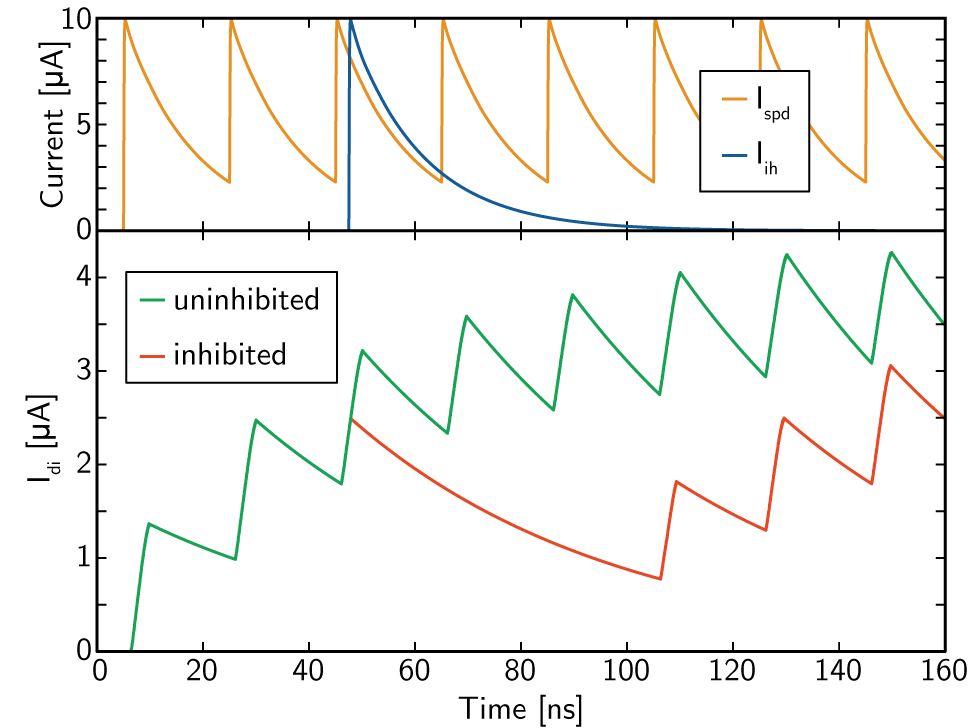
\includegraphics[width=8.6cm]{_09__si_di_inhibition.png}}
	\captionof{figure}{\label{fig:si_di_inhibition}Caption.}
\end{figure}
Simulated operation of a dendrite with a single excitatory and single inhibitory synapse is shown in Fig.\,\ref{fig:si_di_inhibition}. The upper panel shows a temporal trace of excitatory activity, which consists of a pulse train at 20\,MHz. A single inhibitory synapse event occurs shortly after the third pulse of the excitatory train. The lower panel shows the current circulating in the DI loop as a function of time for cases with and without the inhibitory synapse event. Without inhibition, current is added to and decays from the DI loop, as expected. When inhibition occurs, the effect of excitation is immediately quenched, even though the most recent synaptic pulse is still of sufficient amplitude to drive $J_{\mathrm{df}}$ above $I_{\mathrm{c}}$. Immediately following the inhibitory synapse event, $I_{\mathrm{di}}$ begins decaying with time constant $\tau_{\mathrm{di}}$. Inhibition decays with a completely independent time constant, $\tau_{\mathrm{ih}} = L_{\mathrm{ih}}/r_{\mathrm{ih}}$, just as all other loops discussed thus far. When the inhibitory current has decayed sufficiently, the effect of the excitatory pulse train resumes. 

The duration over which the dendrite is inhibited is controlled by $\tau_{\mathrm{ih}}$, and for the network to be rapidly adaptable under the influence of inhibition, this time constant will be as short as a gamma-range interspike interval. If inhibition is required over theta time scales, repeated activity on the inhibitory neuron can keep the dendrite suppressed. However, this may not be the most energy-efficient mode of operation. Given the circuits under consideration, we can utilize a mode of operation complimentary to inhibition. In this configuration, the mutual inductors and bias to the DR loop are chosen so that even with all afferent SI loops saturated, the current across $J_{\mathrm{df}}$ cannot exceed $I_{\mathrm{c}}$. Only when an additional, unique synapse fires does the current exceed $I_{\mathrm{c}}$. The additional synapse is designed to saturate with each synapse event and to decay rapidly, so the action of this synapse is to allow $J_{\mathrm{df}}$ to sample $I_{\mathrm{dr}}$. When this synapse fires, the current generated in the DI loop provides an answer to the question, ``How much current is in the DR loop?'' We refer to neurons making synaptic connections of this type as rapid query neurons. 

\begin{figure} 
    \centering{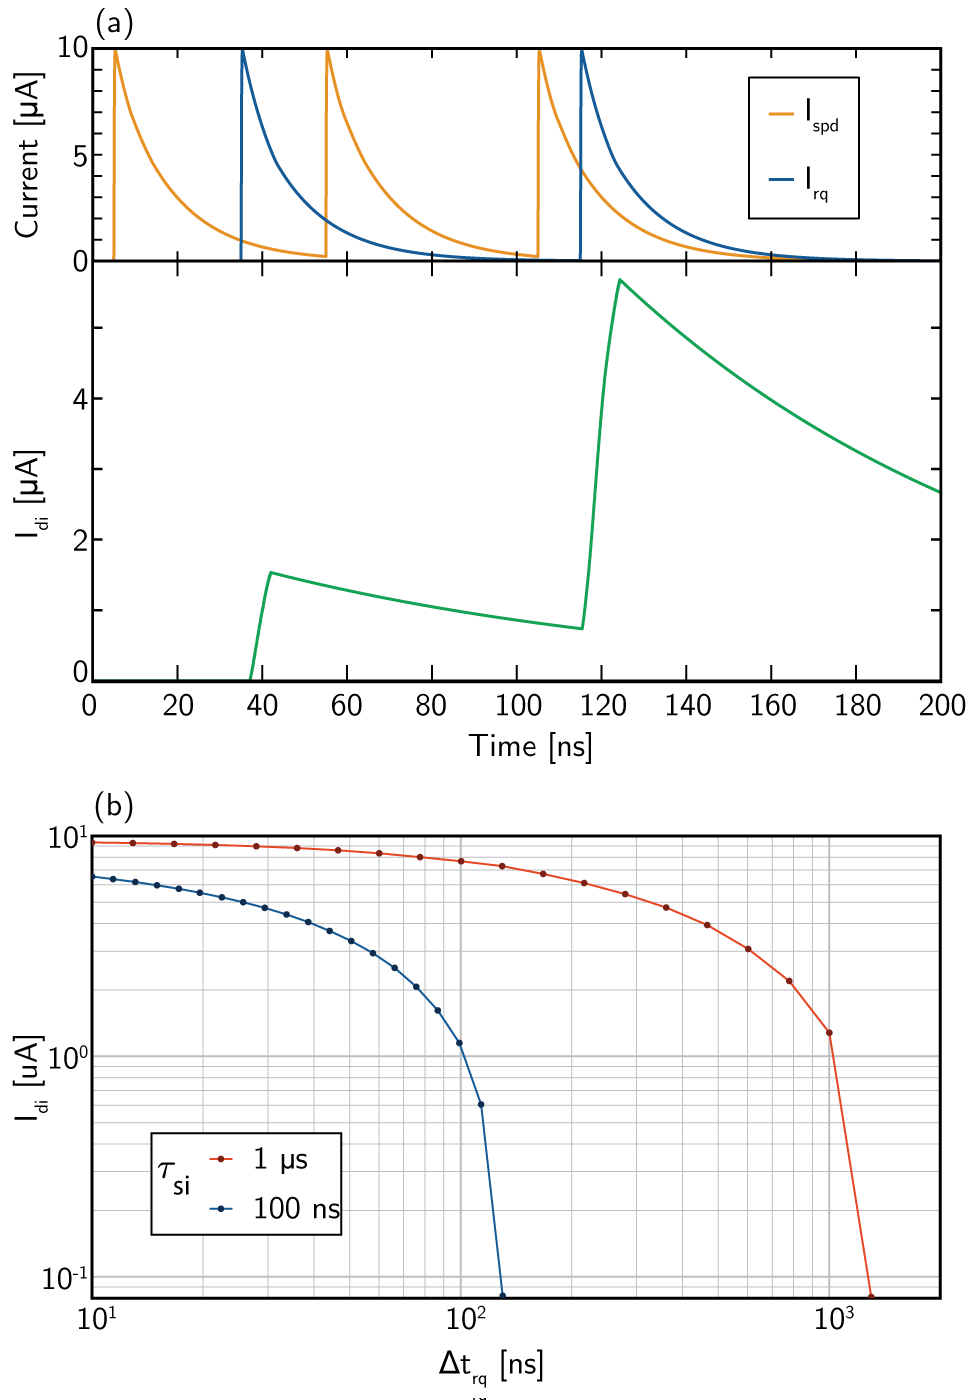
\includegraphics[width=8.6cm]{_10__si_di_rapid_query.png}}
	\captionof{figure}{\label{fig:si_di_rapid_query}Caption. $\tau_{\mathrm{rq}} = 10$\,ns.}
\end{figure}
Figure \ref{fig:si_di_rapid_query} considers rapid query operation. The circuit under consideration comprises a single excitatory synapse and a single rapid query synapse coupled to a DR loop in the configuration of Fig.\,\ref{fig:circuits}(b). In the present example, three excitatory synapse events occur, as seen in the upper panel of Fig.\,\ref{fig:si_di_rapid_query}(a). Two rapid query synapse events are also shown in that panel. The first rapid query event follows the first excitatory pulse by 30\,ns, and with $\tau_{\mathrm{si}} = 20$\,ns, only a small amount of current is added to the DI loop. The second excitatory event is not followed by a rapid query event, and no current is added to DI. The third excitatory event is followed by a rapid query event with 10\,ns delay, and significantly more current is induced in the DI loop. 

The behavior of this circuit is summarized more systematically in Fig.\,\ref{fig:si_di_rapid_query}(b). Here we plot the current induced in the DI loop as a function of the time delay between the rapid query and excitatory events for two values of $\tau_{\mathrm{si}}$. We see that the signal generated by rapid query follows the exponential decay of the SI loop, thus providing an accurate mapping of $I_{\mathrm{si}}$ to $I_{\mathrm{di}}$ at the time rapid query was performed. 

We plot the exponential functions of Fig.\,\ref{fig:si_di_rapid_query}(b) on a log-log graph to emphasize that each SI loop provides information over single time scale determined by $\tau_{\mathrm{si}}$. It would be desirable to find a means by which a memory trace may be extracted across multiple time scales from a single photonic synapse event. This increased temporal dynamic range is one example of what can be achieved if electronic copies of photonic synapse events are produced. This fluxonic fan out is the subject of the next section.

\section{\label{sec:fluxonic_fanout}Fluxonic fan-out from photonic synapses}
In neural systems using light for communication, photons are likely to be the most valuable resource from an energy perspective. We have described many different operations that can be performed to extract information from photonic synapse events and pulse trains, and we would like to perform them all simultaneously without requiring an additional photonic synapse for each. We can straightforwardly copy fluxons with a pulse splitter, a common means of achieving fan out of flux-quantum signals \cite{lise1991}, and we can therefore simply copy the output signals from a single photonic synapse to multiple independent SI loops that can each perform different temporal filters and feed into different dendrites. We refer to these as electronic synapses.

The circuit for splitting pulses is shown in Fig.\,\ref{fig:circuits}(c). A fluxon enters from the left, and when it switches the initial junction, the current of the resulting fluxon is split to two subsequent junctions. These junctions are biased such that the amount of current is sufficient to exceed $I_{\mathrm{c}}$, thus producing fluxons at both junctions with restored signal level. For the application at hand, the splitter of Fig.\,\ref{fig:si_di_rapid_query}(c) can be placed following $J_{\mathrm{jtl}}$ in Fig.\,\ref{fig:si_di_rapid_query}(a) or Fig.\,\ref{fig:si_di_rapid_query}(b). Thus, signals produced by synapses or dendrites can be copied and processed independently to extract distinct information through multiple temporal filters and logical operations. The circuit of Fig.\,\ref{fig:si_di_rapid_query}(c) achieves direct one-to-two fanout. If a greater number of copies is desired, the same circuit can be repeated in a tree. The limits of this fan out will depend on one's tolerance for circuit complexity, a theme we will discuss in Sec.\,\ref{sec:discussion}. We speculate that in mature systems, a given photonic synapse may split to as many as ten electronic synapses. 

\begin{figure} 
    \centering{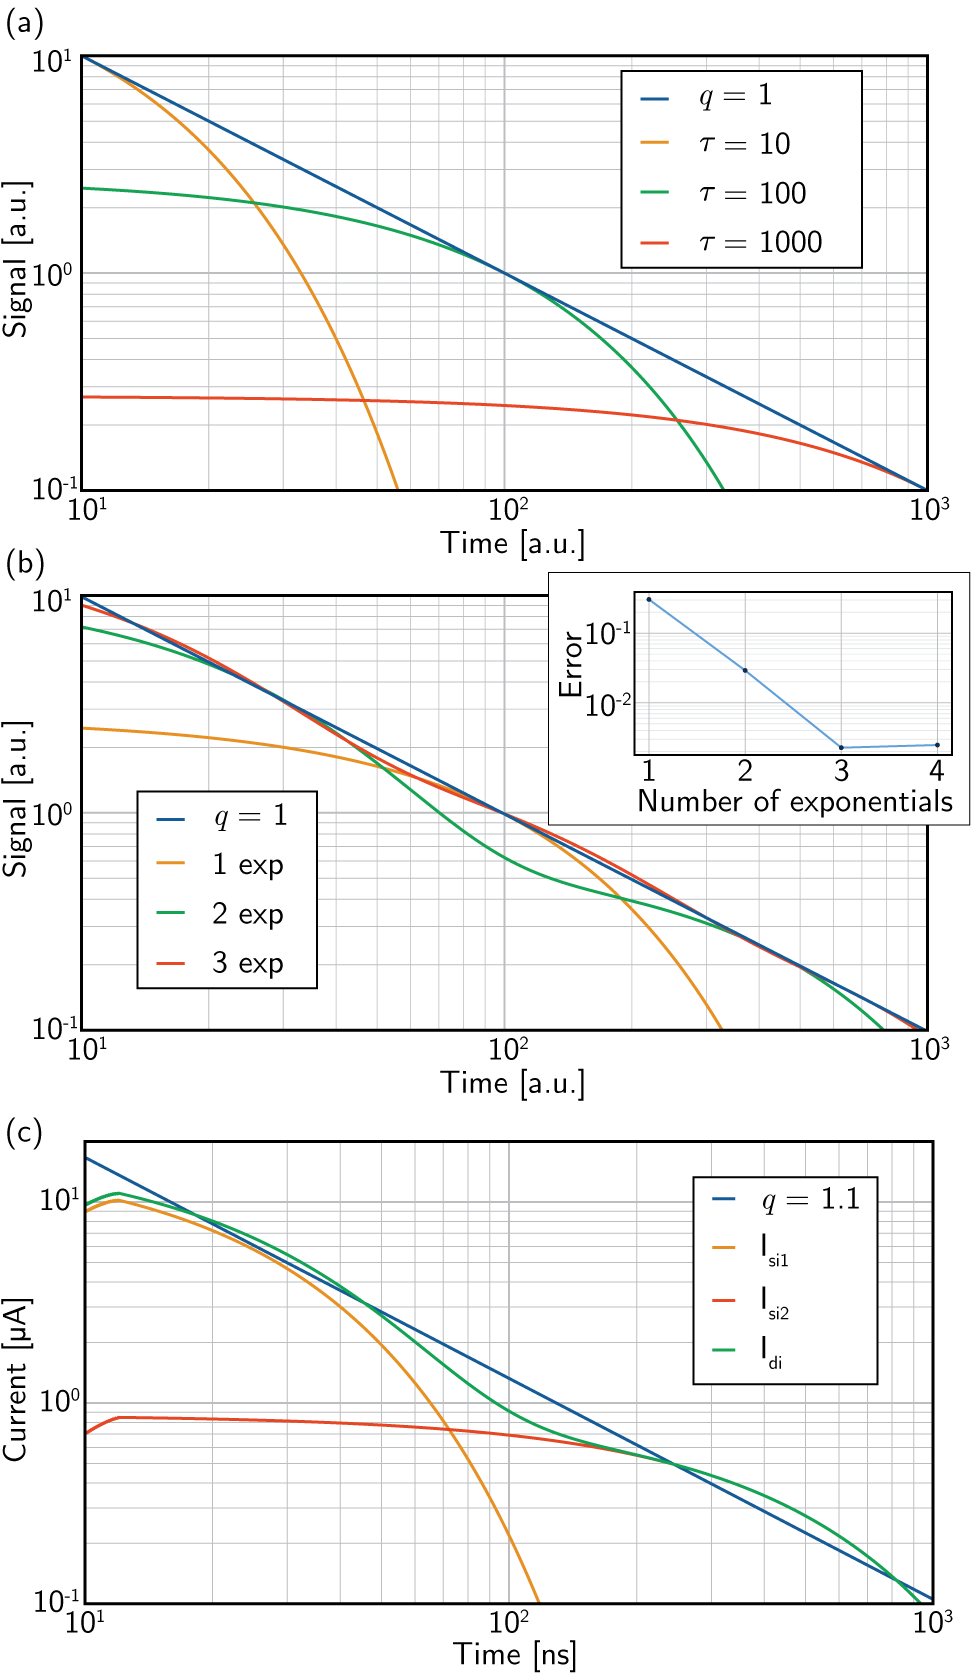
\includegraphics[width=8.6cm]{_11__power_law_time_decay.png}}
	\captionof{figure}{\label{fig:power_law_time_decay}Caption.}
\end{figure}
As a simple example of the utility of pulse splitting, we consider a single photonic synapse feeding into two electronic synapses. Figure \ref{fig:power_law_time_decay}(a) summarizes the motivation. Instead of retaining a memory trace of a synapse event over only a single temporal scale as is present in a single SI loop with exponential decay, we would prefer a signal with a power law decay information across temporal scales can be accessed. In Fig.\,\ref{fig:power_law_time_decay}(a) we compare $f(t) \propto t^{-q}$ to $g(t) \propto e^{-t/\tau}$ for three values of $\tau$. The smallest value of $\tau$ provides no information past its cutoff, and the signal from the largest value of $\tau$ is nearly constant across more than an order of magnitude. The middle value gives a poor representation at the start and the end. Figure \ref{fig:power_law_time_decay}(b) shows that we can obtain a suitable approximation to the power law function by superposing a small number of exponentials. Here we represent a power law with unity exponent, mapping two orders of magnitude in time to two order of magnitude in signal. Convergence is shown in the inset. The error is improved an order of magnitude by using two exponentials instead of one, and there is little advantage to using more than three for this task. 

We implement this principle with the circuits under consideration by copying the signal from a photonic synapse to two electronic synapses coupled to a common passive superconducting loop via mutual inductors. We choose the time constants and couplings of the two SI loops to approximate the fitting technique employed to produce Fig.\,\ref{fig:power_law_time_decay}(b). Figure \ref{fig:power_law_time_decay}(c) shows the current in each of the SI loops as well as the common output loop. A power law with $q = 1.1$ is shown for comparison. This power-law temporal extension can be used in conjunction with many of the other operations discussed thus far, with the objective to use cheap fluxonic operations to extend the memory trace of expensive photonic activity across extra orders of magnitude in time. Such operation performs a power-law mapping of a temporal signal to the dynamic range of the firing junction, and allows a single dendrite to retain and access information regarding gamma and theta frequencies. 

This example of using pulse splitting to access broader time spans is a straightforward extension of the behavior of a single SI loop shown in Fig.\,\ref{fig:sffg_basic}(a). Additional functionality can be envisioned by combining pulse splitting with many of the functions discussed in this paper. But even without these extension, by copying the output from a photonic synapse, each of the operations discussed here can be performed simultaneously. With a single photon, The dendritic tree can be provided with information regarding the synapse's average firing rate across multiple temporal scales; the time since the last synaptic firing; various quantities regarding initiation and duration of pulse trains; coincidences and sequences with synapses from multiple other neurons; and inhibition and rapid query applied independently to each of these pieces of information.

\section{\label{sec:discussion}Discussion}
\begin{itemize}
\item extensions (XOR,...
\item bit depth (all loops are 8 to 10)
\item logic-level restoration
\item the soma is basically just another dendrite at the root of the tree, except it feeds into no DR, but rather the amplifier chain
\item we have only considered binary inhibition. Multiple IH loops could achieve partial inhibition
\item trying to maximize what the dendritic tree knows and can communicate to the neuron
\item fan-out photonic, fan-in electronic
\item fading memory
\end{itemize}



With inhibition, all branches of the dendritic tree are functionally responsive by default and are selectively silenced by inhibitory synapse events. With rapid query, all branches of the dendritic tree are silent by default and are only functionally connected if rapid query synapse events occur. If the information in a given dendrite need not be accessed regularly, rapid query will be more energy efficient than continually performing inhibition. We do not propose rapid query instead of inhibition, but rather in addition. To our knowledge, there is no rapid query neuron in the biological domain. This may be due to a computational inadequacy that we have overlooked, or it may be that the circuits under consideration are more amenable to such a mode of operation, which requires a degree of control over competing circuit parameters. There are dozens of different, specialized neurons in the mammalian brain, with x different types of inhibitiory neurons all playing specific roles \cite{bu2006}. Superconducting optoelectronic networks take significant inspiration from the brain, but hardware discrepancies will inevitably lead to departures in computation. Perhaps rapid query neurons are one such departure, and we hope this hypothesis is tested in time.

\vspace{2em}
This is a contribution of NIST, an agency of the US government, not subject to copyright.
	
\newpage
\appendix
\section{\label{apx:circuit_parameters}Parameters used in circuit simulations}

\bibliographystyle{unsrt}
\bibliography{fluxonic_processing_of_photonic_synapse_events}

\end{document}